\section{Shape Regulation under PCC Approximation}
%
This section provides an example of application of the proposed model augmentation and model-based control strategy for the setpoint regulation of a pneumatically actuated planar soft robot, modeled through \gls{PCC} approximation with acting gravity forces. 

\subsection{Model}\label{sub:backstepping:pcc_model}
\textbf{Background - PCC dynamic model:}
We consider a planar soft robotic arm consisting of three segments analogue to \cite{della2020model} modelled using the \gls{PCC}~\cite{jones2006kinematics} assumption, but the formulation can be easily extended to the 3D case while neglecting the torsional deformations. Alternatively, a strain-based parameterization could be employed~\cite{boyer2020dynamics}. 
% The \gls{PCC}~\cite{jones2006kinematics} assumption stitches together segments each with constant curvature.
We assume a weight distribution of $m_i = \int_{0}^{l_i} \rho_i(s') ds'$ along the center line of the segment $i$. Gravity is acting along the vector $g \in \mathbb{R}^2$. We consider the following equations of motions with diagonal matrices $K$ and $D$:
\begin{equation}\small\label{eq:backstepping:dynamics_pcc_case}\small
\begin{split}
	B(q)\ddot{q} + C(q,\dot{q}) \, \dot{q} + G(q) + K \, q + D \, \dot{q} + G_{\mathrm{P}}^{\mathrm{q}}(q,\mu_\mathrm{p}) &= 0, \\
	M_\mathrm{p} \, \ddot{\mu}_\mathrm{p} + D_\mathrm{p} \, \dot{\mu}_\mathrm{p} + G_{\mathrm{P}}^{\mu_\mathrm{p}}(q,\mu_\mathrm{p}) &= f_\mathrm{p}. \; 
\end{split}
\end{equation}

\textbf{Fluid Volume in Chamber:}
A model of the fluid volume in the chambers as a function of the configuration of the segment is required to evaluate the conservative forces by the fluid as specified in \eqref{eq:backstepping:GPq} and \eqref{eq:backstepping:GPmu}. In this section, we derive a simple analytical model based on \gls{CC} kinematics.
It is assumed that the volume of the chamber is only dependent on the curvature of the segment as we model the segment length $l_{0,i}$ to stay constant and the chambers to be inextensible in radial direction of the curvature. We visualize the model and its parameters in Figure~\ref{fig:backstepping:pcc_case_overview}. Thus, the volume of chamber $j$ part of segment $i$ is defined as:
\begin{equation}\small
    V_{\mathrm{C},j}(q_i) = \int_{d_{\mathrm{C},\mathrm{a},j}}^{d_{\mathrm{C},\mathrm{b},j}} b_\mathrm{C} \, l_i(d_\mathrm{C}') \, \mathrm{d}d_\mathrm{C}',
\end{equation}
where $b_\mathrm{C}$ describes the constant planar thickness of the chamber and $l_i(d'_\mathrm{C})$ the length of segment $i$ at offset $d'_\mathrm{C}$ from the center-line. 
The function $l_i(d'_\mathrm{C})$ is derived by the properties of constant curvature of the segment
\begin{equation}\small
    l_i(d'_\mathrm{C}) = l_{0,i} - q_i d'_\mathrm{C}.
\end{equation}
%We remind ourselves of the relation between radius $r_i$ and curvature $\kappa_i$ of the segment: $r_i = \frac{1}{\kappa_i}$. As the angle between the base and the tip of the segment $q_i = \kappa_i l_i(0)$ stays constant irrespective of offset $d'_\mathrm{C}$, we can relate the lengths:
% \begin{equation}\small
%     q_i = \frac{l_i(0)}{r_i} = \frac{l_i(d'_\mathrm{C})}{r_i-d'_\mathrm{C}},
% \end{equation}
% which leads using $l_{0,i} = l_i(0)$ to
% \begin{equation}\small
%     l_i(d'_\mathrm{C}) = \frac{r_i-d'_\mathrm{C}}{r_i} l_{0,i} = l_{0,i} - q_i d'_\mathrm{C}.
% \end{equation}
% We can use this expression to analytically integrate along $d_\mathrm{C}'$. 
The integration inherits an opposite sign for the change of volume with $q_i$ for the left and right chamber respectively for an inner and outer chamber wall radius of $0 < d_{\mathrm{C},\mathrm{a}} < d_{\mathrm{C},\mathrm{b}} < d_i$ and a continuum segment of radius $d_i$:
%for the volume from an inner wall radial coordinate $d_{\mathrm{C},\mathrm{a},j}$ to an outer wall radial coordinate $d_{\mathrm{C},\mathrm{b},j}$:
\begin{equation}\small
\begin{split}
     V_{\mathrm{C},j}(q_i) = b_\mathrm{C} \left ( l_{0,i} ( d_{\mathrm{C},\mathrm{b}}-d_{\mathrm{C},\mathrm{a}}) \mp \frac{q_i}{2} (d_{\mathrm{C},\mathrm{b}}^2 - d_{\mathrm{C},\mathrm{a}}^2) \right ).
\end{split}
\end{equation}
The partial derivative $\partial_{q} V_{\mathrm{C}}$ is determined as
\begin{equation}\small
    \partial_{q_i} V_{\mathrm{C},j} = \mp \, 0.5 \, b_\mathrm{C} \, (d_{\mathrm{C},\mathrm{b}}^2-d_{\mathrm{C},\mathrm{a}}^2).
\end{equation}
% The gradient inherits an opposite sign for the left and right chamber respectively for an inner and outer chamber wall radius of $0 < d_{\mathrm{C},\mathrm{a}} < d_{\mathrm{C},\mathrm{b}} < d_i$ for a continuum segment of radius $d_i$:
% \begin{equation}\small
%     \partial_{q_i} V_{\mathrm{C}} = \mp 0.5 \, b_\mathrm{C} (d_{\mathrm{C},\mathrm{b}}^2-d_{\mathrm{C},\mathrm{a}}^2).
% \end{equation}

\subsection{Set point control}
% \begin{figure*}[ht]
%   \centering
%   \subfigure[Configuration $q$]{\includegraphics[width=0.33\textwidth]{figures/time_series_plot_configuration_v4.eps}\label{fig:backstepping:time_series_plot_configuration}}
%   \subfigure[Piston position $\mu_\mathrm{p}$]{\includegraphics[width=0.33\textwidth]{figures/time_series_plot_piston_position_v4.eps}\label{fig:backstepping:time_series_plot_piston_position}}
%   \subfigure[Actuation force $f_\mathrm{p}$]{\includegraphics[width=0.33\textwidth]{figures/time_series_plot_actuation_force_v4.eps}\label{fig:backstepping:time_series_plot_actuation_force}}\\
%   \caption{Simulation of posture regulation under \gls{PCC} approximation comparing the performance of the nonlinear backstepping controller (dashed lines) with a PID baseline controller (dotted lines). The set-point reference configuration is shown with solid lines.}
% \end{figure*}
\begin{figure*}[ht]
  \centering
  \captionsetup[subfigure]{labelformat=empty}
  % End-to-end PID
  \subfigure{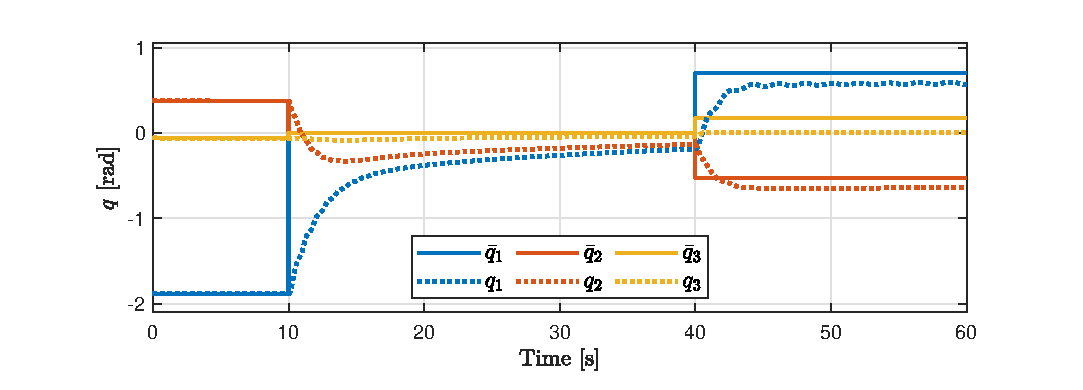
\includegraphics[width=0.32\textwidth, trim={0.75cm 0.87cm 0.75cm 0cm}]{backstepping/figures/time_series_plot_configuration_full_system_PID_v2}}
  \subfigure{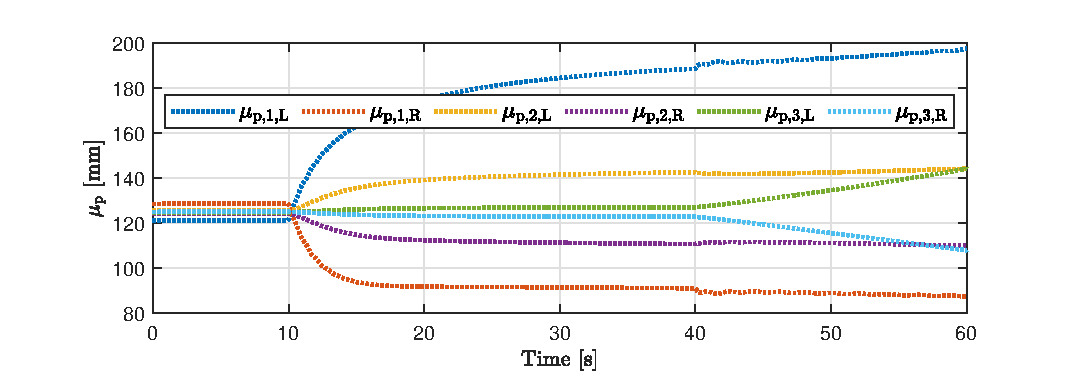
\includegraphics[width=0.32\textwidth, trim={0.75cm 0.87cm 0.75cm 0cm}]{backstepping/figures/time_series_plot_piston_position_full_system_PID_v2.eps}}
  \subfigure{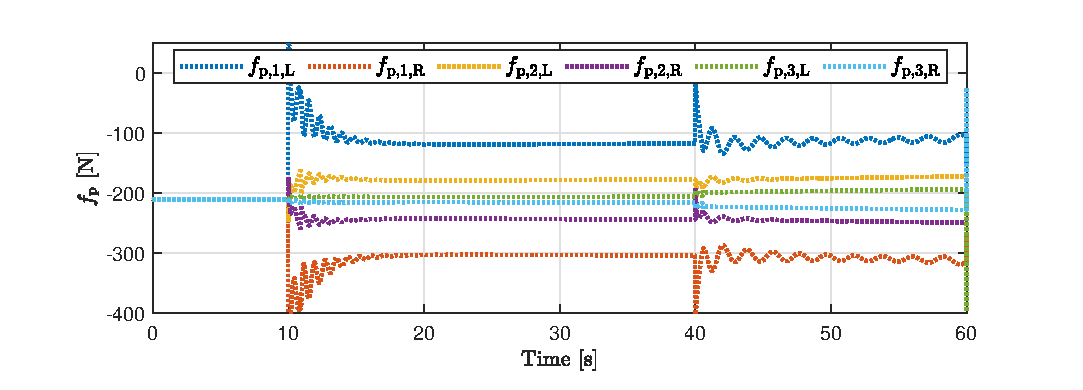
\includegraphics[width=0.32\textwidth, trim={0.75cm 0.87cm 0.75cm 0cm}]{backstepping/figures/time_series_plot_actuation_force_full_system_PID_v2.eps}}\\
  % Coupling-aware PID
  \subfigure{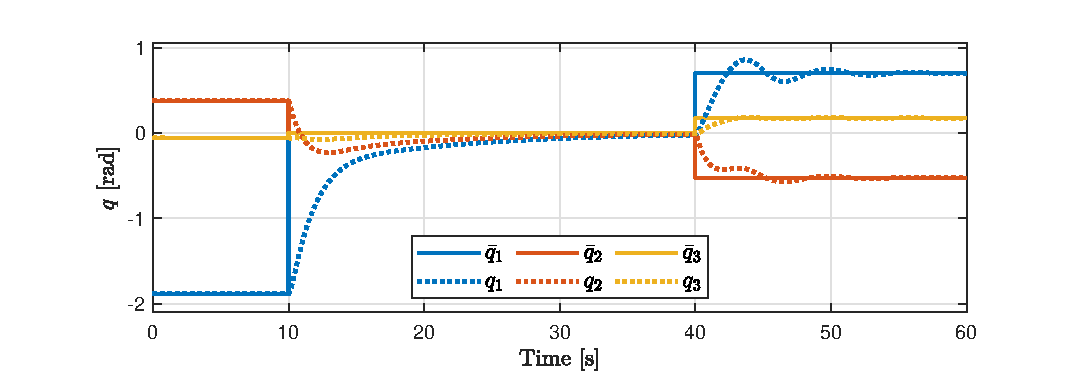
\includegraphics[width=0.32\textwidth, trim={0.75cm 0.87cm 0.75cm 0cm}]{backstepping/figures/time_series_plot_configuration_coupling_aware_PID_v2.eps}}
  \subfigure{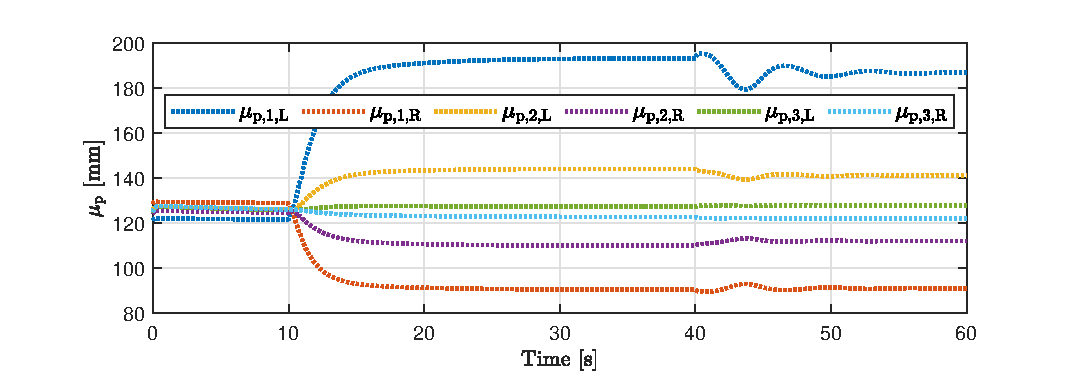
\includegraphics[width=0.32\textwidth, trim={0.75cm 0.87cm 0.75cm 0cm}]{backstepping/figures/time_series_plot_piston_position_coupling_aware_PID_v2.eps}}
  \subfigure{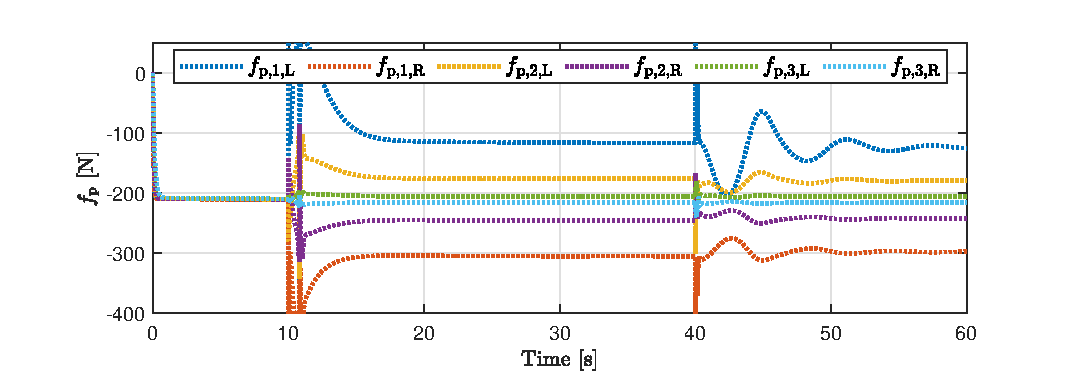
\includegraphics[width=0.32\textwidth, trim={0.75cm 0.87cm 0.75cm 0cm}]{backstepping/figures/time_series_plot_actuation_force_coupling_aware_PID_v2.eps}}\\
  % Backstepping
  \subfigure[Configuration $q$]{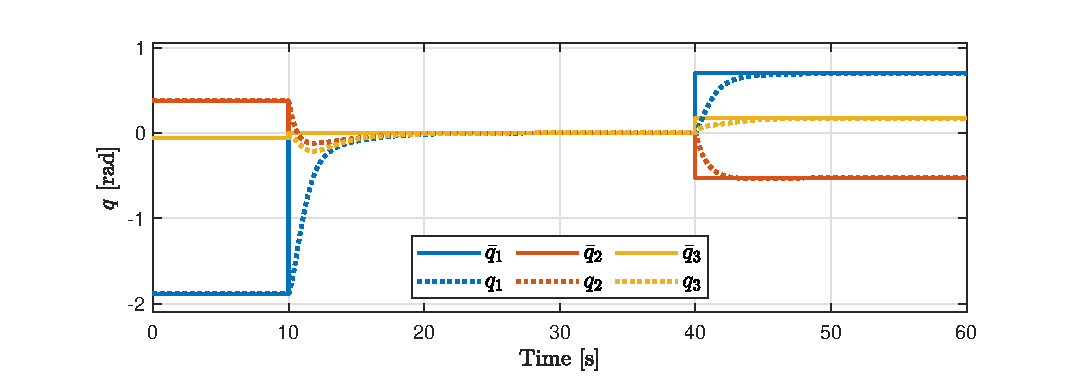
\includegraphics[width=0.32\textwidth, trim={0.75cm 0cm 0.75cm 0cm}]{backstepping/figures/time_series_plot_configuration_backstepping_v2.eps}}
  \subfigure[Piston position $\mu_\mathrm{p}$]{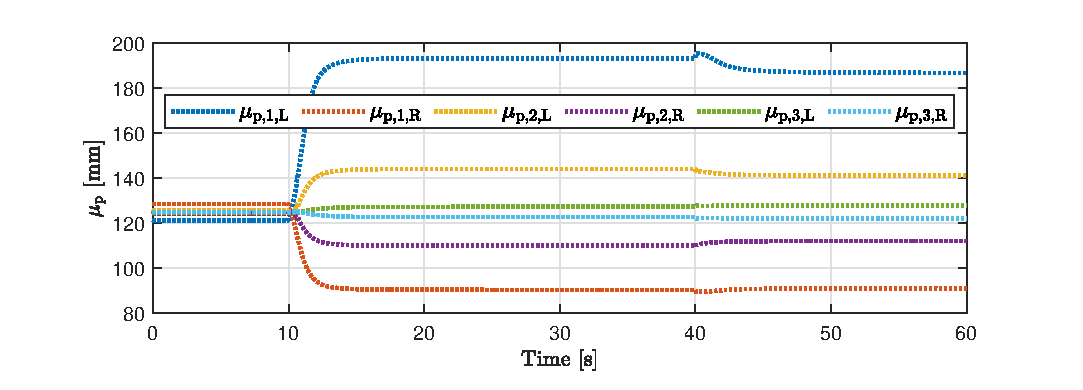
\includegraphics[width=0.32\textwidth, trim={0.75cm 0cm 0.75cm 0cm}]{backstepping/figures/time_series_plot_piston_position_backstepping_v2.eps}}
  \subfigure[Actuation force $f_\mathrm{p}$]{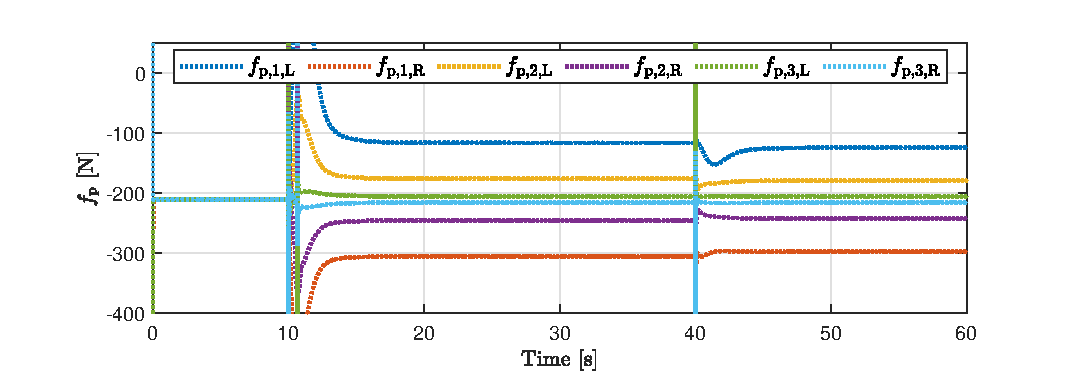
\includegraphics[width=0.32\textwidth, trim={0.75cm 0cm 0.75cm 0cm}]{backstepping/figures/time_series_plot_actuation_force_backstepping_v2.eps}}\\
  \caption{Simulation of posture regulation under \gls{PCC} approximation comparing the performance of an end-to-end PID baseline controller (1st row), with a coupling-aware PID controller (2nd row) and the nonlinear backstepping controller (3rd row). The set-point reference configuration is shown with solid lines.}
  \vspace{-0.5cm}
  \label{fig:backstepping:time_series_plots}
\end{figure*}

\textbf{Configuration-space control:}
%
Consider the following regulator of desired configuration $\Bar{q} \in \mathbb{R}^{n_\mathrm{q}}$, 
%
\begin{equation}\small\label{eq:backstepping:high_level_regulation}
    \Bar{\tau}(q, \Bar{q}) = K \Bar{q} + G(q),
\end{equation}
%
where $\Bar{\tau} \in \mathbb{R}^{n_\mathrm{q}}$ is the torque in configuration space. %This will be our high level controller $\Gamm(q)$ as 
%
% This leads to the following equations of motion for the system: %
% \begin{equation}\small
%      B(q) \Ddot{q} + C(q, \dot{q}) \dot{q} = K (\Bar{q} - q) + D (-\dot{q}),
% \end{equation}
% which is essentially a PD controller with gravity compensation. 
Asymptotic stability of the equilibrium $\Bar{q}$ is proven through the Lyapunov function $H(q, \dot{q}) = \dot{q}^{\mathrm{T}} B(q) \dot{q}/2 + q^\mathrm{T} K q/2$, which yields the time derivative $\dot{H} = -\dot{q}^\mathrm{T} D \dot{q}/2 \leq 0$.

\textbf{Mapping from configuration to actuation space with force balance:}
Our backstepping controller requires access to $\Gamma(q,\dot{q})$ which returns a desired piston $\bar{\mu}_\mathrm{p}$ given the desired torque $\bar{\tau}$ and the current state of the soft system $(q,\dot{q})$. In the planar case with inextensible segments, there exist a redundancy in actuating the pistons controlling the pressure in the left and right chambers of a segment to trigger $\bar{\tau}$ on the segment. Thus, we decide to solve this redundancy by equally attributing the desired torque to both pistons.

We assume that the system is calibrated at a straight configuration $q_{\mathrm{t}0} = 0$ with pistons preloaded at position $\mu_{p,t0} \in \mathbb{R}^{n_{\mu_\mathrm{p}}}$ leading to a fluidic volume of
 \begin{equation}\small
     V_{\mathrm{t}0,j} = V_{\mathrm{C},j}(q_{\mathrm{t}0,i}) + \mu_{\mathrm{p},\mathrm{t}0,j} \, A_{\mathrm{p},j}
 \end{equation}
 % and causing a fluidic pressure of $p_{\mathrm{t}0,j} = p_\mathrm{atm} \frac{V_{\mathrm{C},j}(q_i=0) + l_{\mathrm{p},j} A_{\mathrm{p},j}}{V_{\mathrm{C},j}(q_i=0) + \mu_{\mathrm{p},\mathrm{t}0,j} A_{\mathrm{p},j}}$ 
in the system. After preloading, the fluids in the left and right chambers each apply a preloaded torque of magnitude $G_{\mathrm{P},\mathrm{t}0}^{q} \in \mathbb{R}^{n_\mathrm{q}}$ on the soft system.
% \begin{equation}\small
%     G_{\mathrm{P},\mathrm{t}0,i}^{q} =
%     -p_\mathrm{atm} \partial_{q_i} V_{\mathrm{C},j} A_{\mathrm{p},j} \frac{l_{\mathrm{p},j} - \mu_{\mathrm{p},\mathrm{t}0,j}}{V_{\mathrm{t}0,j}}.
% \end{equation}
It is implicitly assumed that the piston length $l_\mathrm{p}$, piston area $A_\mathrm{p}$, the preloaded piston position $\mu_{\mathrm{p},\mathrm{t}0}$ and the preloaded volume $V_{\mathrm{t}0}$ are equal for the left and right chambers of segment $i$.
We can write the conservative forces acting on the left chamber $G_{\mathrm{P},\mathrm{L}}^q(q, \mu_\mathrm{p}) \in \mathbb{R}^{n_\mathrm{q}}$ and right chamber $G_{\mathrm{P},\mathrm{R}}^q(q, \mu_\mathrm{p}) \in \mathbb{R}^{n_\mathrm{q}}$ as differences from the neutral conservative force $G_{\mathrm{P},\mathrm{t}0}^{q}$
\begin{equation}\small
\begin{split}
    G_{\mathrm{P},\mathrm{L}}^q = G_{\mathrm{P},\mathrm{t}0}^{q} + \Delta G_{\mathrm{P},\mathrm{L}}^q,
    \quad
    G_{\mathrm{P},\mathrm{R}}^q = - G_{\mathrm{P},\mathrm{t}0}^{q} + \Delta G_{\mathrm{P},\mathrm{R}}^q.
\end{split}
\end{equation}
% \begin{equation}\small
% \begin{split}
%     G_{\mathrm{P},\mathrm{L}}^q(q, \mu_\mathrm{p}) &= G_{\mathrm{P},\mathrm{t}0}^{q} + \Delta G_{\mathrm{P},\mathrm{L}}^q(q, \mu_\mathrm{p}),\\
%     G_{\mathrm{P},\mathrm{R}}^q(q, \mu_\mathrm{p}) &= - G_{\mathrm{P},\mathrm{t}0}^{q} + \Delta G_{\mathrm{P},\mathrm{R}}^q(q, \mu_\mathrm{p}).
% \end{split}
% \end{equation}
The force applied by the fluid in the left and right chambers on the system is
\begin{equation}\small
    G_{\mathrm{P}}^q(q, \mu_p) =  G_{\mathrm{P},\mathrm{L}}^q + G_{\mathrm{P},\mathrm{R}}^q = \Delta G_{\mathrm{P},\mathrm{L}}^q + \Delta G_{\mathrm{P},\mathrm{R}}^q .
\end{equation}
We re-arrange to find an expression for the desired conservative force offsets which equally distribute a commanded torque $\Bar{\tau}$ to the fluid in both chambers. Setting
$\Delta \Bar{G}_{\mathrm{P},\mathrm{L}}^{\Bar{q}} =  \Delta \Bar{G}_{\mathrm{P},\mathrm{R}}^{\Bar{q}} = 0.5 \, \Bar{\tau}(q, \Bar{q})$
% \begin{equation}\small
%      \Delta \Bar{G}_{\mathrm{P},\mathrm{L}}^{\Bar{q}} =  \Delta \Bar{G}_{\mathrm{P},\mathrm{R}}^{\Bar{q}} = 
%      % -\frac{\Bar{\tau}}{2},
%      0.5 \, \Bar{\tau}(q, \Bar{q}),
% \end{equation}
results for the chosen set point controller $\Bar{\tau}$ and a diagonal elastic matrix $K$ with elements $k_i$ in:
\begin{equation}\small\label{eq:backstepping:dist_G_p_q_planar_pcc}
    \Bar{G}_{\mathrm{P},j}^{\Bar{q}}(q, \Bar{q}_i) 
    % = \pm G_{\mathrm{P},\mathrm{t}0,i}^{q} - 0.5 \Bar{\tau}_i 
    = \pm G_{\mathrm{P},\mathrm{t}0,i}^{q} - 0.5 \left ( k_i \Bar{q}_i + G_i(q) \right ).
\end{equation}
\eqref{eq:backstepping:GPq} is inversed to compute the desired piston position $\Bar{\mu}_{\mathrm{p}} = \Gamma(q, \Bar{q})$:
\begin{equation}\small\label{eq:backstepping:gamma}
    \Gamma_j(q, \Bar{q}) = \frac{1}{A_{\mathrm{p},j}} \left ( \frac{\alpha_{\mathrm{air},j} \, \partial_{q_i} V_{\mathrm{C},j}}{p_\mathrm{atm} \, \partial_{q_i} V_{\mathrm{C},j} - \Bar{G}_{\mathrm{P},j}^{\Bar{q}}(q, \Bar{q})} - V_{\mathrm{C},j}(q) \right ).
\end{equation}
\textbf{Backstepping:}
The system is now in the form of \eqref{eq:backstepping:reduced_sys}, so Theorem~1 can be invoked and a specialized version of \eqref{eq:backstepping:pi_psi} can be derived for the \gls{PCC}-case and our chosen set-point controller of \eqref{eq:backstepping:high_level_regulation}. The partial derivative of the Lyapunov function of the soft system controller evaluates to $ \partial_{\dot{q}} H(q, \dot{q}) = \dot{q}^\mathrm{T} B(q)$, which allows to re-formulate \eqref{eq:backstepping:pi_psi} into:
\begin{equation}\small
\begin{split}
    \Pi &= \dot{\Gamma} - K_1 (\mu_p - \Gamma) + S^\mathrm{T} \dot{q},\\
    \Psi &= G_{\mathrm{P}}^{\mu_\mathrm{p}} + D_\mathrm{p} \, \Pi + M_\mathrm{p} \, \dot{\Pi} - K_2 \, (\dot{\mu}_\mathrm{p} - \Pi) - (\mu_\mathrm{p} - \Gamma).
\end{split}
\end{equation}

% \textbf{Backstepping to piston velocity:} 
% To complete the backstepping to the piston velocity $\Pi(q, \dot{q})$, we require access to the time derivative of the \gls{PCC} controller in actuation space $\dot{\Gamma}(q, \Bar{q}, \dot{q}) = \partial_q \Gamma (q, \Bar{q}) \dot{q}$:
% \begin{equation}\small
%     \dot{\Gamma}_j = \frac{1}{A_{\mathrm{p},j}} \left ( \frac{\alpha_{\mathrm{air},j} \partial_{q_i} V_{\mathrm{C},j} \partial_{q} \Bar{G}_{\mathrm{P},j}^{\Bar{q}}}{\left ( p_\mathrm{atm} \partial_{q_i} V_{\mathrm{C},j} - \Bar{G}_{\mathrm{P},j}^{\Bar{q}} (q, \Bar{q}) \right )^2} - \partial_{q} V_{\mathrm{C},j} \right ) \dot{q}.
% \end{equation}
% For the proposed set point controller, we can subsequently also determine the partial derivative of the commanded force $\partial_q \Bar{G}_{\mathrm{P},j}^{\Bar{q}}(q, \Bar{q}) = - 0.5 \, \partial_q G_i(q)$.
% The partial derivative of the Lyapunov function of the soft system controller evaluates to $ \partial_{\dot{q}} H(q, \dot{q}) = \dot{q}^\mathrm{T} B(q)$, which allows us to re-formulate \eqref{eq:backstepping:pi_psi}:
% \begin{equation}\small\label{eq:backstepping:pi_pcc_set_point}
%     \Pi(q, \Bar{q}, \dot{q}, \mu_\mathrm{p}) = \dot{\Gamma} - K_1 (\mu_p - \Gamma) + S^\mathrm{T} \dot{q}.
% \end{equation}
% \textbf{Backstepping to piston force:}
% We require access to the time derivative of the controller $\Pi(q, \dot{q})$:
% \begin{equation}\small
%     \dot{\Pi}(q, \Bar{q}, \dot{q}, \mu_\mathrm{p}, \dot{\mu}_\mathrm{p}) = \partial_q \Pi \dot{q} + \partial_{\dot{q}} \Pi \Ddot{q} + \partial_{\mu_\mathrm{p}} \Pi \dot{\mu}_\mathrm{p},
% \end{equation}
% and substitute $\Ddot{q} = f(q, \dot{q}) + g(q, \mu_\mathrm{p})$ as accelerations are hard to measure in reality
% \begin{equation}\small
% \begin{split}
%     \dot{\Pi} = & -K_1 \left ( \dot{\mu}_\mathrm{p} - \dot{\Gamma}(q, \Bar{q}, \dot{q}) \right ) + \left ( \partial_q \dot{\Gamma} + \dot{S}^\mathrm{T} \right ) \dot{q}\\
%     & + \left ( \partial_{\dot{q}} \dot{\Gamma} + S^\mathrm{T} \right ) \left ( f(q,\dot{q}) + g(q,\mu_\mathrm{p}) \right ) .
% \end{split}
% \end{equation}
% We define the final controller of the required piston force $\Bar{f}_\mathrm{p}$
% \begin{equation}\small
% \begin{split}
%     & \Bar{f}_\mathrm{p} = \Psi(q, \Bar{q}, \dot{q}, \mu_\mathrm{p}, \dot{\mu}_\mathrm{p})\\
%     & \Psi = G_{\mathrm{P}}^{\mu_\mathrm{p}} + D_\mathrm{p} \, \Pi + M_\mathrm{p} \, \dot{\Pi} - K_2 \, (\dot{\mu}_\mathrm{p} - \Pi) - (\mu_\mathrm{p} - \Gamma).
% \end{split}
% \end{equation}